\documentclass[10pt,a4paper,titlepage]{report}
\usepackage[latin1]{inputenc}
\usepackage{amsmath}
\usepackage{amsfonts}
\usepackage{amssymb}
\usepackage[labelfont=bf]{caption}
\usepackage{float}
\usepackage{listings}
\usepackage[section]{placeins}
\usepackage{graphicx}
\usepackage[left=2cm,right=2cm,top=2cm,bottom=2cm]{geometry}
\usepackage{tikz}
\usepackage[intoc, english]{nomencl}
\makenomenclature
\author{Elijah Andrews}
\title{Implementing the Discrete Element Method with OpenCL for GPUs}
\makeindex
\begin{document}
\tableofcontents
\chapter*{Abstract}
\addcontentsline{toc}{chapter}{Abstract}
\nomenclature{$\mathbf{u}$}{Particle Velocity Vector}
\nomenclature{$\mathbf{u}_n$}{Relative Velocity Normal to Collision}
\nomenclature{$\delta$}{Particle Body Surface Overlap Distance}
\nomenclature{$\delta_{e}$}{Particle Effect Surface Overlap Distance}
\nomenclature{$\mathbf{F}$}{Force}
\nomenclature{$\mathbf{F}_n$}{Normal Contact Force}
\nomenclature{$\mathbf{F}_t$}{Tangential Contact Force}
\nomenclature{$\mathbf{F}_c$}{Cohesion Force}
\nomenclature{$\mathbf{F}_g$}{Gravitational Force}
\nomenclature{$\mathbf{F}_d$}{Drag Force}
\nomenclature{$\eta$}{Damping Coefficient}
\nomenclature{$\mathbf{\hat{n}}$}{Collision Normal Unit Vector}
\nomenclature{$\mathbf{\hat{t}}$}{Collision Tangent Unit Vector}
\nomenclature{$\mu$}{Friction Coefficient}
\nomenclature{$\zeta$}{Tangential Displacement During Interaction}
\nomenclature{$k_e$}{Normal Collision Stiffness}
\nomenclature{$k_f$}{Friction Stiffness}
\nomenclature{$k_c$}{Cohesion Stiffness}
\nomenclature{$t$}{Time}
\nomenclature{$O_p$}{Particle Origin}
\nomenclature{$s_b$}{Particle Body Surface}
\nomenclature{$s_e$}{Particle Effect Surface}
\nomenclature{$d_b$}{Particle Body Surface Diameter}
\nomenclature{$d_e$}{Particle Effect Surface Diameter}
\nomenclature{$N$}{Number of Particles}
\nomenclature{$\mathbf{u}_f$}{Fluid Velocity Vector}
\nomenclature{$\mathbf{g}$}{Gravitational Acceleration Vector}
\nomenclature{$\tau_p$}{Particle Relaxation Time}
\nomenclature{$d_p$}{Particle Diameter}
\nomenclature{$\rho_p$}{Particle Density}
\nomenclature{$\mu$}{Dynamic Viscosity}
\nomenclature{$u$}{Particle Speed}
\nomenclature{$u_{0}$}{Initial Particle Speed}
\nomenclature{$\mathbf{x}$}{Particle Position Vector}
\printnomenclature
\chapter{Introduction}
\section{Project Overview}
\textit{What the project is about, why it is significant etc.}
\section{Project Goals}
Thus the aim of this project is to implement the DEM for large numbers of particles on OpenCL. This will allow for an assessment of OpenCL performance with large numbers of particle that has not yet been tested.
\\\textit{$<$ Currently just a copy-paste from interim report, this will be expanded on and more clearly defined later on. $>$}
\section{Report Structure}
This report has three main parts. Firstly, the model being used and its numerical implementation are discussed. Chapter \ref{ch:The Discrete Element Method} provides detail on the mathematical model and the analytic equations of motion for the model. Chapter \ref{ch:Numerical Methods} shows how the mathematical model is implemented numerically and has some comparisons of method accuracy.
\\The second part explains how the model is implemented programmatically. Chapter \ref{ch:Python Implementation} discusses the initial implementation of the algorithm in Python. Chapter \ref{ch:OpenCL Implementation} contains a background in Graphics Processing Units and how OpenCL functions. It also discusses the details of the final OpenCL implementation. Both of these chapters contain relevant simulation verification test cases.
\\The final part is the application of the simulation to the study of how agglomerates form with varying particle properties and initial conditions. This demonstrates the capabilities of the simulation and provides some useful insights.
\section{Previous Work}
The project directly preceding this one was 'Programming GPU Cards with OpenCL to Predict the Motion of Billions of Particles'\cite{achow} by Andrew Chow. His project developed a parallelised particle-fluid simulator using OpenCL. Particle-particle interactions were not considered in his project. This project will expand upon his by implementing particle-particle interactions using the Discrete Element Method.
\\The DEM has been implemented many times since it was originally devised by Cundall in 1971\cite{cundallphd}. Improvements in the algorithm have been proposed and implemented, and it has proven to be a reliable technique.
\\Many implementations have been CPU based with no parallelisation, but in recent years implementations have tended to be parallelised. The vast majority of parallel DEM implementations\cite{blazedem}\cite{GAN20161172}\cite{demcuda1}\cite{demcuda2}\cite{demcuda3} have used NVIDIA's CUDA platform which is restricted to running on NVIDIA GPUs. This means that these implementations are not usable on other hardware. One solution to this problem is to use the Open Computing Language (OpenCL). OpenCL code can be executed across heterogeneous platforms. This includes CPUs, GPUs and other, more novel, processing units. This means that an implementation programmed in OpenCL can be accessible to most users. One paper described an implementation that did use OpenCL but the application was for a real-time interactive simulation and so relatively low numbers of particles were used (16,000 was the maximum benchmarked)\cite{kinect}. Another paper briefly describes an adaptation of a simple existing implementation and its performance, however testing, decision, and implementation details are not extensive and testing was only done with $2^{17}$ (131,072) particles\cite{washizawa}.
\\This project draws from the work of Rob Tuley whose PhD thesis\cite{tuley} outlined some of the key aspects of the DEM as well as its application in powder simulations.
\\\textit{$<$ A lot of this was from interim report. I'm concerned that it may be too much detail on previous DEM implementations before DEM is explained properly. $>$}
\section{Single Particle Motion in Fluids}
\label{sec:Single Particle Motion in Fluids}
\textit{This is just a summary of what Andrew Chow did, should I just include a sentence about what he did in the Previous Work section? I think this is useful because a lot of the non-DEM stuff was based heavily on what he did so a decent understanding of what he did lends to the background of what I'm doing.\\}
The focus of the previous project was simulating how a particle moves in a fluid. The governing equations from that project form the basis of this project. The governing equation of motion was equation \ref{eq:single particle motion} where $\mathbf{u}$ is the particle velocity, $\mathbf{u}_f$ is the fluid velocity at the particle location, $\tau_p$ is the particle relaxation time, and $\mathbf{g}$ is the gravitational acceleration.
\begin{equation}
\label{eq:single particle motion}
\dfrac{d\mathbf{u}}{dt} = \dfrac{1}{\tau_p}(\mathbf{u} - \mathbf{u}_f) + \mathbf{g}
\end{equation}
The particle relaxation time, $\tau_p$ is an approximate timescale describing how the particle's velocity changes in a fluid due to drag. Assuming Stoke's Law drag on a spherical particle, $\tau_p$ can be defined by equation \ref{eq:particle relaxation time} where $\rho_p$ is the particle density, $d_p$ is the particle diameter, and $\mu$ is the dynamic viscosity of the fluid.
\begin{equation}
\label{eq:particle relaxation time}
\tau_{p} = \dfrac{\rho_{p} d^{2}_{p}}{18 \mu}
\end{equation}
\chapter{The Discrete Element Method}
\label{ch:The Discrete Element Method}
\textit{$<$ I'm considering adding an overall algorithm flowchart somewhere in this chapter. $>$}
\\The Discrete Element Method (DEM) is a numerical method for simulating how particles move and interact. The general principle is that individual particles of a medium are treated as separate rather than making continuum assumptions. This makes it a good method for modelling behaviours in granular materials such as sand, grain, or powder. The DEM can be implemented with either soft or hard collision models. Soft models allow for overlap and treat collisions as sustained events whereas hard models treat collisions as an instantaneous event and model forces as an impulse. Soft collision models have broader applicability as they model sustained contact and multiple simultaneous collisions as well as some other complex phenomena\cite{softvshard}. For this reason a soft contact model has been chosen for this project.
\section{Particle Definition}
The DEM can be used with arbitrary polyhedra, however for simplicity this project will only consider spherical particles as defined in figure \ref{fig:particle} where $O_p$ is the particle origin, $s_b$ is the body surface, and $s_e$ is the effect surface. The diameters of the particle body surface and particle effect surface are denoted by $d_b$ and $d_e$, respectively.
\begin{figure}[!ht]
\centering
\usetikzlibrary{shapes.misc}

% From http://tex.stackexchange.com/questions/123760/draw-crosses-in-tikz
\tikzset{cross/.style={cross out, draw=black, fill=none, minimum size=2*(#1-\pgflinewidth), inner sep=0pt, outer sep=0pt}, cross/.default={2pt}}

\begin{tikzpicture}

\draw  (0,0) node (v1) {} ellipse (1 and 1);
\draw [dashed] (v1) ellipse (1.5 and 1.5);
\node at (0.75,0) {$s_b$};
\node at (1.75,0) {$s_e$};
\node at (-0.15,-0.25) {$O_p$};
\draw (0,0) node[cross] {};
\end{tikzpicture}
\caption{Definition of a particle.}
\label{fig:particle}
\end{figure}
\section{DEM Forces}
\label{sec:DEM Forces}
The Discrete Element Method can simulate a number of different forces using a variety of models. The merits of some of the most common models are discussed in Tuley\cite{tuley}. For this project the simplest force models have been chosen to reduce the overall complexity of the simulation.
\subsection{Normal Contact Force}
In a real elastic collision there will be some deformation of the particles. Calculating the deformation itself would be computationally expensive and would not be of interest in the study of particle population behaviours. The interaction can be modelled as a linear spring-dashpot arrangement where the overlap between the two particles is the compression of the spring. The damping is based on the relative velocity in the normal direction. The force is thus described by equation \ref{eq:normal contact force} where $k_{e}$ is the collision stiffness, $\delta$ is the particle overlap, $\mathbf{\hat{n}}$ is the unit vector normal to the collision, $\eta$ is the damping coefficient, and $\mathbf{u}_{n}$ is the normal velocity.%TODO Make this clearer.
\begin{equation}
\mathbf{F}_{n} = k_{e} \delta \mathbf{\hat{n}} - \eta \mathbf{u}_{n}
\label{eq:normal contact force}
\end{equation}
\subsection{Tangential Contact Force}
The tangential contact force is the friction between two particle surfaces. There are two regimes of friction force, static and dynamic. In the static regime there is no tangential motion and the friction acts to stop motion. In the dynamic regime two surfaces are sliding across one another and the friction acts to arrest this motion. The static regime usually has a higher friction coefficient than the dynamic regime. The simplest and least computationally expensive model for friction is a 'complex friction model'. This calculates values for both of the regimes and applies the minimum of the two calculations.\cite{tuley}
\\\\The static regime friction force is calculated with equation \ref{eq:static friction} where $k_f$ is the friction stiffness, $\zeta$ is the tangential displacement during the interaction, and $\mathbf{\hat{t}}$ is the unit vector tangential to the collision. 
\begin{equation}
\mathbf{F}_{t}^{static} = - k_{f} \zeta \mathbf{\hat{t}}
\label{eq:static friction}
\end{equation}
\\The dynamic regime friction force is calculated with equation \ref{eq:dynamic friction} where $\mu$ is the coefficient of friction.
\begin{equation}
\mathbf{F}_{t}^{dynamic} = - \mu |\mathbf{F}_{n}| \mathbf{\hat{t}}
\label{eq:dynamic friction}
\end{equation}
\\The final tangential friction force is defined in equation \ref{eq:friction force}.
\begin{equation}
\mathbf{F}_{t} = -\mathbf{\hat{t}}min(|\mathbf{F}_{t}^{static}|, |\mathbf{F}_{t}^{dynamic}|)
\label{eq:friction force}
\end{equation}
\subsection{Cohesion Force}
Cohesion is the attractive force between two bodies of the same material, adhesion is the attractive force between two bodies of different materials. For this project all of the particles and walls are assumed to be of the same material and so only cohesion is considered, however adhesion could be modelled using varying cohesion stiffnesses. Although there are many complex effects that could be considered\cite{tuley}, a basic linear approximation can be used to model a cohesion force. This is defined in equation \ref{eq:cohesion force} where $k_c$ is the cohesion stiffness and $\delta_e$ is the particle effect surface overlap.
\begin{equation}
\mathbf{F}_{c} = k_{c} \delta_{e} \mathbf{\hat{n}}
\label{eq:cohesion force}
\end{equation}
\section{Equations of Motion}
The motion of particles in the simulation is governed by equation \ref{eq:acceleration}. This is derived from Newton's Second Law of motion. The total force, $\mathbf{F}$ is a combination of forces as shown in equation \ref{eq:total force}. $\mathbf{F}_{n}$, $\mathbf{F}_{t}$, and $\mathbf{F}_{c}$ are the forces defined in section \ref{sec:DEM Forces}. $\mathbf{F}_{g}$ and $\mathbf{F}_{d}$ are the gravitational force and drag force, respectively, and are defined in section \ref{sec:drag and gravity}.
\begin{equation}
\dfrac{d\mathbf{x}}{dt} = \mathbf{u}
\label{eq:position}
\end{equation}
\begin{equation}
\dfrac{du}{dt} = \dfrac{\mathbf{F}}{m}
\label{eq:acceleration}
\end{equation}
\begin{equation}
\mathbf{F} = \mathbf{F}_{n} + \mathbf{F}_{t} + \mathbf{F}_{c} + \mathbf{F}_{g} + \mathbf{F}_{d}
\label{eq:total force}
\end{equation}
\subsection{Drag and Gravitational Forces}
\label{sec:drag and gravity}
The drag force is the same as that used in the previous project. Equation \ref{eq:drag force} defines the drag force from the acceleration used in equation \ref{eq:single particle motion}.
\begin{equation}
\label{eq:drag force}
\mathbf{F}_{d} = \dfrac{m}{\tau_p} (\mathbf{u}_f - \mathbf{u})
\end{equation}
The gravity force is also the same as that used in the previous project and is defined in equation \ref{eq:gravitational force}.
\begin{equation}
\label{eq:gravitational force}
\mathbf{F}_{g} = m \mathbf{g}
\end{equation}
\section{Useful Results}
\subsection{Reduced Mass}
When considering the motion of two particles relative to each other a useful property is the reduced mass. Consider the relative acceleration of two particles in a collision. To determine the relative acceleration between the two particles, the two accelerations must be combined. It is known that $F_1$ and $F_2$ are equal and opposite. Finding the relative acceleration results in equation \ref{eq:relative acceleration}. This provides a relationship between the force in a collision and the relative acceleration as a result of that collision. It is of a similar form as Newton's Second Law but with the usual mass replaced with the reduced mass of the two particles (equation \ref{eq:reduced mass}). This reduced mass can be used instead of particle mass in equation \ref{eq:acceleration} when considering relative motion of particles.
\begin{align}
F_1 &= m_1 a_1 \nonumber
\\F_2 &= m_2 a_2 \nonumber
\\F_1 &= -F_2 \nonumber
\\a_{rel} &= a_2 - a_1 \nonumber
\\&= \dfrac{F_2}{m_2} - \dfrac{F_1}{m_1} \nonumber
\\&= \dfrac{F_2}{m_2} + \dfrac{F_2}{m_1} \nonumber
\\&= F_2 \Big(\dfrac{1}{m_2} + \dfrac{1}{m_1}\Big) \nonumber
\\&= F_2 \Big(\dfrac{m_1 + m_2}{m_1 m_2}\Big) \nonumber
\\F_2 &= \Big(\dfrac{m_1 m_2}{m_1 + m_2}\Big) a_{rel} \label{eq:relative acceleration}
\\m_{reduced} &= \dfrac{m_1 m_2}{m_1 + m_2} \label{eq:reduced mass}
\end{align}
It should be noted that equation \ref{eq:reduced mass} reduces to $m_1$ if $m_2$ tends to infinity. This is useful when considering static particles with infinite density and is used extensively for verifying simulation results (see section \ref{sec:verification}).
\subsection{Collision Duration}
\subsection{Coefficient of Restitution}
\section{Rotation/Quaternions}
\textit{$<$This will be completed later as it is not immediately relevant to the progress of the project.$>$}
\section{Collision Detection}
A key part of the DEM is effective collision detection. If approached naively collision detection is simply calculating the overlap for every particle with every other particle. This is extremely inefficient and causes the simulation to run in $O(N^2)$ time, where $N$ is the number of particles. To improve efficiency this process can be split into two phases. Firstly, the broad phase determines which particles could collide with which other particles. This reduces the number of particle collisions that have to be calculated. The second phase, collision resolution, resolves the collisions by measuring overlap. The goal of the broad phase is to allow the simulation to run in $O(N)$ time.
\\There are many different algorithms that can be used for broad phase collision detection, varying in complexity and efficiency. Although some of the more complex algorithms were considered, the gain in efficiency was not significant enough to outweigh the significant increase in implementation complexity. For this reason the simplest algorithm, spatial zoning, has been chosen for this project.
\\Spatial zoning separates the simulation domain into control volumes. Particles are then sorted into the control volumes. Particles in neighbouring, or the same, control volumes are then resolved fully. It is most efficient to have the control volumes as small as possible because this reduces the number of particles in neighbouring control volumes. Control volumes must be at least as large as the largest particle in the simulation to ensure that neighbouring control volumes contain all possible collisions. For monodisperse particle populations this means that the control volumes should be the same size as the particles. For polydisperse particle populations this means that the control volumes should be the size of the largest particle in the population. As mentioned in Tuley\cite{tuley} this can decrease efficiency for statistical distributions of particle sizes. Sections \ref{sec:Python Collision Detection} and \ref{sec:OpenCL Collision Detection} provide further detail as to how this is implemented computationally in Python and with OpenCL, respectively.
\chapter{Numerical Methods}
\label{ch:Numerical Methods}
\section{Numerical Integration Schemes}
The DEM model used in this project has stiff governing equations. This means that the simulation may become unstable if the timestep is not sufficiently small. Thus, the choice of integration scheme is important. For simplicity, there are three main schemes that will be considered for this project: the Euler method (or forward Euler method), the backward Euler method (or implicit Euler method), and the trapezoidal rule.
\\The forward Euler method is an explicit integration method, using the current value to estimate the next value. It has first order accuracy and requires only the data from the current iteration.
\\The backward Euler method is an implicit integration method, assuming the next value and solving the equation for it. It also has first order accuracy and requires only the data from the current iteration.
\\The trapezoidal rule is an implicit integration method that uses the average of the current and next values. It has second order accuracy.
\\For the implicit methods either an analytic solution to the implicit equations or a numerical solution can be used. For simplicity, only the functions that can form analytic solutions from the implicit equations will use the implicit methods.
\subsection{Velocity}
For equation \ref{eq:acceleration} the forward Euler method for integrating acceleration to get velocity at iteration n is shown in equation \ref{eq:Forward Euler Acceleration}. In this case the force, $F$, is a function of $u_n$.
\begin{equation}
u_{n+1} = u_{n} + \dfrac{F(u_n)}{m}\Delta t
\label{eq:Forward Euler Acceleration}
\end{equation}
\\For the same equation, the backward Euler method is shown in equation \ref{eq:Backward Euler Acceleration}. In this case the force, $F$, is a function of $u_{n+1}$.
\begin{equation}
u_{n+1} = u_{n} + \dfrac{F(u_{n+1})}{m}\Delta t
\label{eq:Backward Euler Acceleration}
\end{equation}
For the DEM the total force is a combination of forces (see equation \ref{eq:total force}). Drag and gravity forces are only calculated once per iteration and so can be calculated at the same time as the velocity. However, collision forces are calculated multiple times per iteration to get contributions from all collisions and so cannot be easily calculated at the same time as the velocity. For this reason, the normal force, tangential force, and cohesion force are treated as fixed at the time of velocity calculation. Gravity is also fixed and so equation \ref{eq:total force} can be represented as in equation \ref{eq:force at iteration}. $F(u)$ can then be used in equation \ref{eq:Forward Euler Acceleration} or \ref{eq:Backward Euler Acceleration}.
\begin{equation}
F(u) = F_n + F_t + F_c + F_g + F_d(u)
\label{eq:force at iteration}
\end{equation}
\textit{To be continued... Further derivations of the final equations used and explanations therein.}
\subsection{Position}
Equation \ref{eq:position} is a very simple differential equation that can be solved by integrating. Since the velocity does not directly depend on the position, and the velocity for the next iteration is calculated before the position, it is trivial to use the trapezoidal rule to calculate position. It has all of the advantages of accuracy without the disadvantage of increased complexity. The position can thus be calculated with equation \ref{eq:iterative position}.
\begin{equation}
x_{n+1} = x_n + \dfrac{u_n + u_{n+1}}{2}\Delta t
\label{eq:iterative position}
\end{equation}
\section{Scheme Performance}
\subsection{Comparison of Integration Schemes}
\textit{This section will contain a comparison of explicit and implicit integration schemes. I've temporarily removed the current work on it because it isn't clear.}
%There are three different methods of integrating drag. Firstly, there is the analytical solution, this is the exact solution to the model but cannot be done easily computationally. Secondly, there is the explicit numerical solution, this takes the current state and estimates the future state. Thirdly, there is the implicit numerical solution, this assumes the future state and integrates accordingly.
%For a simple system with constant flow speed and no gravity, the system acceleration is described by equation \ref{eq:drag_acceleration}.
%\begin{equation}
%\dot{u} = \dfrac{v-u}{\tau}
%\label{eq:drag_acceleration}
%\end{equation}
%Equation \ref{eq:drag_acceleration} can be solved to show that the analytical solution for the particle speed, $u$, is that in equation \ref{eq:analytical_drag_speed}.
%\begin{equation}
%u(t) = v(1 - e^{-\dfrac{t}{\tau}})
%\label{eq:analytical_drag_speed}
%\end{equation}
%The explicit numerical integration method for equation \ref{eq:drag_acceleration} is that in equation \ref{eq:explicit_drag_speed}. Where $u_{n}$ is the current speed and $u_{n+1}$ is the speed after timestep $\Delta t$.
%\begin{equation}
%\dfrac{u_{n+1} - u_{n}}{\Delta t} = \dfrac{v - u_{n}}{\tau}
%\label{eq:explicit_drag_speed}
%\end{equation}
%The implicit numerical integration method for equation \ref{eq:drag_acceleration} is that in equation \ref{eq:implicit_drag_speed}. Where $u_{n}$ is the current speed and $u_{n+1}$ is the speed after timestep $\Delta t$.
%\begin{equation}
%\dot{u} = \dfrac{u_{n+1} - u_{n}}{\Delta t} = \dfrac{v - u_{n+1}}{\tau}
%\label{eq:implicit_drag_speed}
%\end{equation}
%Equation \ref{eq:implicit_drag_speed} can be rearranged to get an equation of the form $\dot{u} = f(u_{n})$ as shown in equation \ref{eq:implicit_drag_acceleration}.
%\begin{equation}
%\dot{u} = \dfrac{v - u_{n}}{\tau + \Delta t}
%\label{eq:implicit_drag_acceleration}
%\end{equation}
%When these three methods are applied to the system they produce the results in figure \ref{fig:particle_speed_for_different_integrations}.
%\begin{figure}[!ht]
%\centering
%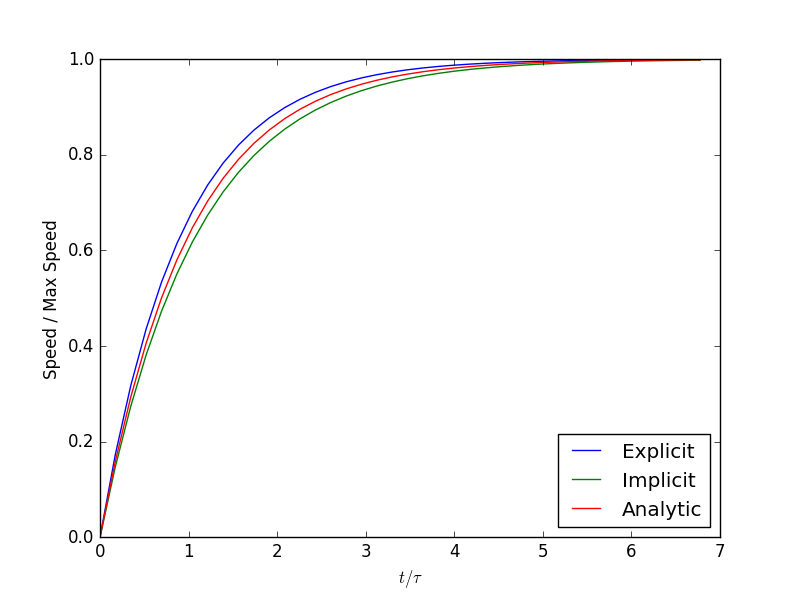
\includegraphics[scale=0.75]{figures/ParticleSpeedWithVaryingIntegration.png}
%\caption{A graph of particle speed against time for the three methods of integration.}
%\label{fig:particle_speed_for_different_integrations}
%\end{figure}
%\\Comparing the explicit and implicit numerical integration to the analytical solution shows that the explicit method has an average percentage difference of 2.05\% and the implicit method has an average percentage difference of 1.85\% when the timestep is $0.1 s$.
%\\The average percentage difference can be compared between the two methods with varying timesteps as shown in figure \ref{fig:avg_percent_diff_against_timestep}. This graph shows that the explicit method increases its average percentage difference approximately linearly with increasing timestep. The implicit method increases its average percentage difference non-linearly at a slower rate than the explicit method. This implies that the implicit method is more accurate than the explicit method, especially for higher timesteps.
%\begin{figure}[!htb]
%\centering
%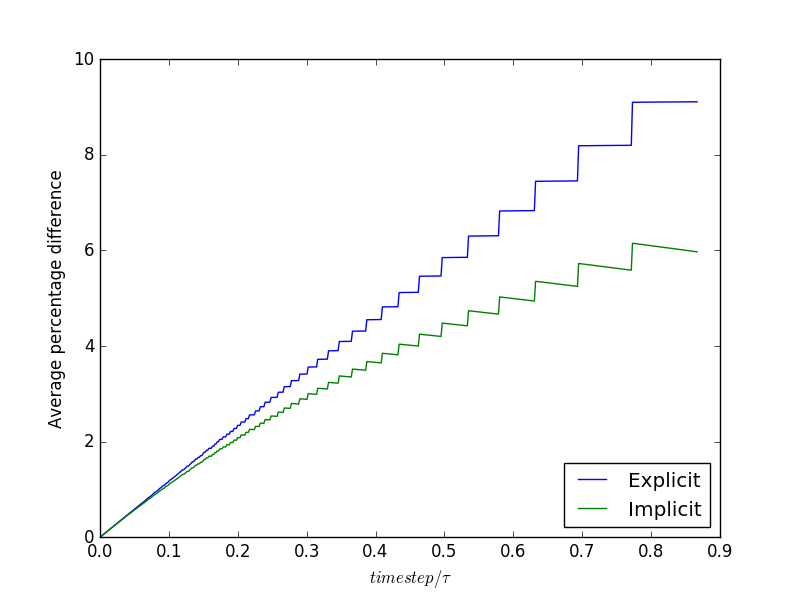
\includegraphics[scale=0.75]{figures/AveragePercentageDifferenceAgainstTimestep.png}
%\caption{A graph of average percentage difference between the numerical method and analytical solution against varying timestep. The jaggedness of the lines is due to the discrete changes in timestep causing small rounding errors.}
%\label{fig:avg_percent_diff_against_timestep}
%\end{figure}
%\\Unlike the explicit method, the implicit method depends on the other accelerations in the system. Equation \ref{eq:implicit_drag_acceleration} can be redefined to include these other accelerations as an extra $\dot{u}_{e}$ term as shown in equation \ref{eq:drag_acceleration_with_other_accelerations}.
%\begin{equation}
%\dot{u} = \dfrac{u_{n+1} - u_{n}}{\Delta t} = \dfrac{v - u_{n+1}}{\tau} + \dot{u}_{e}
%\label{eq:drag_acceleration_with_other_accelerations}
%\end{equation}
%As before, equation \ref{eq:drag_acceleration_with_other_accelerations} can be rearranged to be in the form $\dot{u} = f(u_{n})$ as shown in equation \ref{eq:implicit_drag_acceleration_with_other_accelerations}. The derivation of this can be found in appendix \ref{sec:implicit_drag_accel_derivation}.
%\begin{equation}
%\dot{u} = \dfrac{v - u_{n} + \tau \dot{u}_{e}}{\tau + \Delta t}
%\label{eq:implicit_drag_acceleration_with_other_accelerations}
%\end{equation}
%Equation \ref{eq:implicit_drag_acceleration_with_other_accelerations} can be applied to a particle falling under the effect of gravity through a stationary fluid. The results are shown in figure \ref{fig:fig:terminal_velocity_implicit_explicit}. As with the previous system, the explicit method has an average percentage difference of 2.05\% and the implicit method has an average percentage difference of 1.85\% when the timestep is $0.1 s$. This shows that the accuracy of the modified equation is consistent with that of equation \ref{eq:implicit_drag_acceleration}.
%\begin{figure}[!htb]
%\centering
%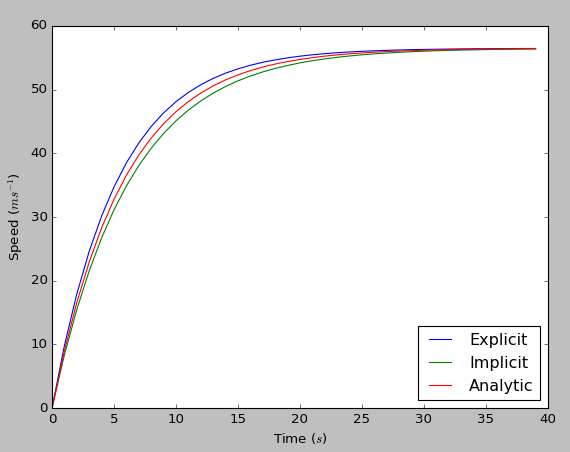
\includegraphics[scale=0.75]{figures/TerminalVelocityImplicitExplicit.png}
%\caption{A graph of particle speed against time for each method of integration using equation \ref{eq:implicit_drag_acceleration_with_other_accelerations}.}
%\label{fig:fig:terminal_velocity_implicit_explicit}
%\end{figure}
\subsection{Timestep Stability}
\textit{This will examine timestep stability. I've temporarily removed the current work on it because it isn't clear.}
%\section{Numerical Integration} \label{sec:Numerical Integration}
%\subsection{Velocity}
%Velocity is iterated with equation \ref{eq:particle_velocity_iteration} where $\dot{u}$ is the acceleration obtained from the function call 'Particle.get{\_}accel()'.
%\begin{equation}
%u_{n+1} = u_{n} + \dot{u} \Delta t
%\label{eq:particle_velocity_iteration}
%\end{equation}
%\subsection{Position}
%Position is iterated with equation \ref{eq:particle_position_iteration}.
%\begin{equation}
%x_{n+1} = x_{n} + \dfrac{u_{n+1} + u_{n}}{2}\Delta t 
%\label{eq:particle_position_iteration}
%\end{equation}
\section{Selected Iterative Functions}
\textit{This section will provide a summary of all of the iterative functions used. This may not be necessary because these will be defined in previous sections. The only reason this section might exist is if a summary is useful to clarify it all.}
\section{Verification}
\label{sec:verification}
\subsection{Drag}
\subsection{Normal Collision}
\subsection{Friction Sliding}
\subsection{Cohesion Collision}
\chapter{Python Implementation}
\textit{The majority of this is disorganised. The main point is that the structure will be:
\\- Overview (general overview of what and why)
\\- Program Structure (Implementation details)
\\- Optimization and Performance (How well the simulation works and measures taken to make it better)
\\- Verification (Verification of the simulation implementation)}
\label{ch:Python Implementation}
\section{Overview}
An initial implementation of the Discrete Element Method has been done in Python. The objective of this implementation is to gain an understanding of the DEM and any inherent computational difficulties. Python has been chosen as a testing environment for its simplicity and ease of development. 
\section{Program Structure}
\subsection{Element Types}
Different element types are required for different types of geometry and particle. For the Python implementation the two simplest have been chosen, a spherical particle and an axis-aligned wall.
\subsubsection{Particle}
The basic particle element is a spherical particle with pre-determined properties. These properties include initial position, initial velocity, diameter, density, fluid viscosity, and functions for fluid velocity and gravity. All of these properties can be set upon instantiation of each particle object and so can be easily modified for a variety of different simulations.
\\There are two objects for particles, the main object, 'Particle', tracks a full particle state history which is very memory intensive and unnecessary for most applications. The second object, 'LowMemParticle', inherits from 'Particle' and only keeps track of the current state and, during iteration, one future state.
\\The particle is iterated using the function call 'Particle.iterate()'. This passes a $\Delta t$ to the particle object and iterates the velocity and position. The methods used for integrating these properties are discussed in section \ref{sec:Numerical Integration}.
\subsubsection{Axis-Aligned Simple Wall}
The basic wall element is an axis-aligned simple wall. This object is defined by two points, minimum and maximum, that must lie in the same plane. From them a rectangle is formed. A normal is calculated for the wall and stored in the object to save time in collision calculations. The wall is treated as fixed, eliminating the need for complex material properties or calculation of motion.
\subsection{Collisions}
\subsubsection{Collision Detection}
\label{sec:Python Collision Detection}
Broad phase collision detection uses the simple spatial zoning technique described in Tuley\cite{tuley}. This approach has been chosen because it is quick and simple to implement. Other options were considered for this implementation but the benefits of using them were far outweighed by the complexity that using them would add to the overall algorithm. Since the initial Python implementation will not be fast anyway it was not deemed necessary to implement optimised algorithms at this stage.
\\The domain is represented by a three dimensional array where each entry is a control volume. The control volume is a list of particles in its bounds. The list of particles is iterated over and each particle assigns itself to the correct control volume. This results in a three dimensional array where each control volume has all of the particles within its bounds as an array. Collision objects are then created for each pair of particles in the same, or neighbouring, control volumes. This approach reduces the problem from $O(N^{2})$ to almost $O(N)$ as shown in figure \ref{fig:run_time_against_N_python}.
\begin{figure}[!ht]
\centering
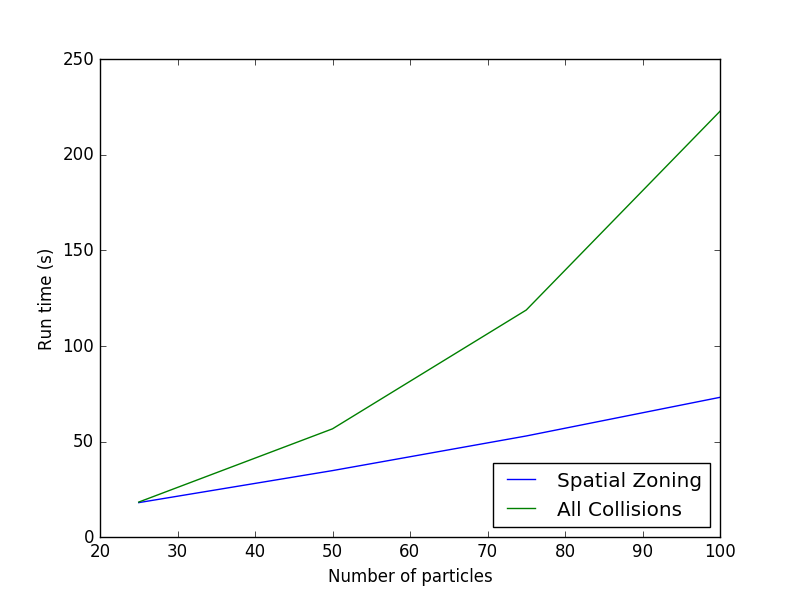
\includegraphics[scale=0.75]{figures/RunTimeAgainstNumberOfParticlesPython.png}
\caption{This graph shows that the simple spatial zoning technique reduces the problem from $O(N^{2})$ down to almost $O(N)$.}
\label{fig:run_time_against_N_python}
\end{figure}
\subsubsection{Collision Resolution}
After an array of collisions has been generated they are iterated over and each collision is resolved. First, the distance between particles is calculated to determine if they are in contact. Often this reveals that they are not in contact and the calculation ends there. If particles are in contact then collision forces are determined.
\\In this initial Python implementation only the simple normal and tangential contact forces are calculated. These are enough to run sufficient initial test cases.
\subsection{Calculating Forces}
There are three categories of forces used in this implementation. These are drag (particle-fluid interaction), gravity, and DEM forces.
\subsubsection{Drag}
The drag forces are determined using Stokes' law as discussed in %TODO Reference
This is calculated using a flow field calculation function that is passed into the Particle object upon instantiation. The particle then calls this function as part of its get\_accel() function. This allows a variety of flow field functions to be used without modifying the Particle object code. The default for this function is a perfectly stationary flow.
\subsubsection{Gravity}
Gravity is treated in a similar manner to drag. A gravity function can be passed into the Particle object upon instantiation. Although this defaults to a simple -9.81$ms^{-2}$, it can be chosen to simulate a rotating frame of reference or other complex configurations. A rotating frame of reference has been implemented in the ``gravity\_shift\_closed\_box'' example simulation. %TODO Reference github
\subsubsection{DEM Forces}
The DEM forces that are calculated in collisions are stored in an array within the Particle object. When the particle is iterated the array is added together and used in the integration calculation. After this calculation the array is cleared so that forces don't get incorrectly added multiple times. This configuration makes it simple to add and remove forces to the simulation whenever necessary and could also be used in general to add any force to the particle.
\section{Verification}
To asses the accuracy of the implementation a series of cases have been tested and compared to analytical solutions of the model.
\subsection{Settling Overlap}
In this case two particles are used. The first particle is an ordinary particle acting under the effects of gravity. The second particle, placed below the first particle, is a particle with quasi-infinite density without being affected by gravity. As time increases the first particle bounces on the second particle until it eventually comes to rest with some overlap with the second particle.\\
\begin{figure}[!htb]
\centering
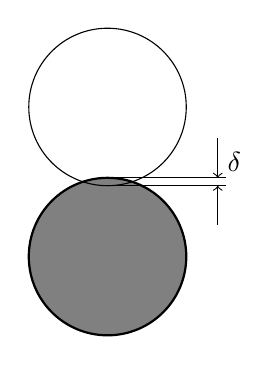
\begin{tikzpicture}
\filldraw[color=black, fill=gray, thick] circle (1);
\draw  (0, 1.9) circle (1);
\draw (0, 1) -- (1.5, 1);
\draw (0, 0.9) -- (1.5, 0.9);
\draw[->] (1.4, 1.5) -- (1.4, 1);
\draw[->] (1.4, 0.4) -- (1.4, 0.9);
\filldraw[black] (1.4, 1.2) node[anchor=west] {$\delta$};
\end{tikzpicture}
\caption{A particle, under the effect of gravity, resting upon a second particle of infinite density, unaffected by gravity. Overlap, $\delta$, is labelled and exaggerated for clarity.}
\end{figure}
\\For the particle to be at rest the particle's gravity must be equal to the normal force from the DEM.
\begin{equation}
F_{g} = F_{n}
\end{equation}
\begin{equation}
mg = k_{e}\delta - \eta u
\end{equation}
To get an equation for overlap, $\delta$, the equation is simplified and rearranged. The speed, $u$, is 0 at rest.
\begin{equation}
\delta = \dfrac{mg}{k_{e}}
\end{equation} 
Taking particle diameter to be 0.1 $m$ and particle density to be 2000 $kg m^{-3}$, the particle mass is 1.047 $kg$. Gravity is taken to be 9.81 $m s^{-2}$ and model spring stiffness is $10^{5}$.
\begin{equation}
\delta = \dfrac{1.047 * 9.81}{10^{5}} = 1.027 * 10^{-4}
\end{equation} 
Running a simulation with these parameters also yields an overlap of $1.027 * 10^{-4}$. Comparing simulation results with high precision overlap prediction shows that the simulation result is within $2.1 * 10^{-11}\%$ of the predicted value.
\subsubsection{Timestep stability}
This result can also be compared for varying timesteps to asses the stability of the implementation. Figure \ref{fig:overlap_percentage_error_against_timestep} shows very stable results up until a timestep of approximately 0.00097.
\begin{figure}[!htb]
\centering
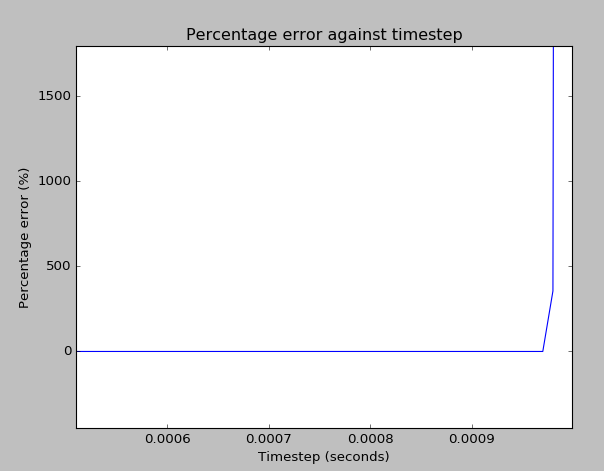
\includegraphics[scale=0.75]{figures/ParticleBounceTimestepAgainstPercentageError.png}
\caption{A graph of overlap percentage error against time step.}
\label{fig:overlap_percentage_error_against_timestep}
\end{figure}
\subsection{Timestep Stability}
Collisions go boom if timestep is too high etc. %<Test against bouncing or something>
The stiffer the collisions the smaller the timestep must be to maintain physical results.
This can be spotted and logged if $E_{k}$ is higher after collision than before.
%TODO Run a simulation of timestep against stiffness.
\section{Optimization and Performance}
\chapter{OpenCL Implementation}
\label{ch:OpenCL Implementation}
\textit{This chapter follows a very similar structure to the Python Implementation chapter.}
\section{OpenCL and Graphics Processing Units}
\textit{This section will briefly explain what a GPU is, what the benefits of using one are, and how OpenCL fits into the whole picture.}
\section{Overview}
\section{Program Structure}
\subsection{Data Structures}
As the C language does not support objects, the objects used in the Python implementation must be simplified into data structures and separate functions. Most of the calculations that were done in the object functions will now be done within the kernels.
\subsubsection{Particle}
The particle structure contains very similar information as the Python implementation particle object. Notable differences are the lack of 'next\_$<$property$>$' variables since these are just used within the iterate\_particle kernel and do not need to be stored.
\\The structure is aligned to the nearest 128 bytes of memory to make accessing it easier. This does waste a little under half of this memory but for $10^7$ particles the particle array requires a total of 1.2GB which is within workable limits.
\subsubsection{Collision}
The collision structure contains two particle IDs and collision properties. This could be reduced to just particle IDs if collisions were taken as having the same properties throughout the simulation. Alternatively, if the collision changed based on particle properties, the collision resolution kernel could calculate the collision properties when they are needed.
\subsubsection{Buffers}
To access the data from the device it must be passed into a buffer. None of the structure data is passed into the buffer so the device must have the same definition of the structure as the host. This is problematic as the host and device have different compilers. To work around this problem the host and device structures are written with members in descending order of size. In addition padding has been added to the host code %TODO Make sure this is the case
 since the alignment specifier is apparently insufficient to ensure correct alignment. The alignment attribute specifier is also not the same between different compilers so ``if defined'' statements are implemented for both Visual Studio and GCC compilers.
\subsection{Kernels}
The main calculations for this implementation are performed on the device. This means that the program must be separated into kernels to be passed over sets of data.
\subsubsection{Collision Detection}
\label{sec:OpenCL Collision Detection}
To improve efficiency, in both speed and resource usage, performing naive collision detection is not viable for large numbers of particles. To improve on this the spatial zoning technique is used similar to the initial Python implementation. However, C does not make arrays of varying sizes easy or efficient so the data structures used and the algorithm implementation must be significantly different.
\\The basic problem is how to store control volumes as lists of references to particles. In Python this was easy, a simple 3D array of control volumes with lists of particle objects inside was sufficient. Various approaches to solving this problem were considered. One approach was to encode particle IDs (equal to the index of a particle in the particles array) with a hashing function into a single number that could be turned back into particle IDs on the device. However, this approach was infeasible because the numbers would get so large that they could not be stored accurately or efficiently.
\\The approach used is to have multiple passes of assignment of particles to control volumes. The first pass simply counts how many particles are in each control volume. This is stored in a single dimensional array of control volumes represented by integers of how many particles each contains. From this array another array is created. This array is of all the particle IDs but sorted into control volumes. The control volumes are of lengths defined by the count array and start at indexes stored in a third array. If a control volume has no particles, the start index of the array is set to -1. For the unsigned long data type this overflows to the maximum value (approximately 4.3 billion) which will likely never be used to index particles. When creating collisions this assumption will be checked and a warning issued. This arrangement of arrays is shown in figure \ref{fig:cv_array_structure}.
\\This approach is somewhat similar to how memory is handled on a computer, but using indexes instead of pointers. For an entirely host-side method an array of pointers to arrays of particles could be used, but this would not be sensible when dealing with device memory as each array would need to be moved to the device before use. Having three arrays that hold all the necessary properties simplifies the memory buffer process significantly. The maths required for turning positions and control volume coordinates into indexes in these arrays are contained in cvUtils.c and kernelUtils.cl for host and device, respectively.
\begin{figure}[!ht]
\centering
\usetikzlibrary{patterns}
\begin{tikzpicture}


\draw [pattern=horizontal lines][help lines, step=1cm] (-5,-1) node (v19) {} grid (4,0) node (v60) {};

\node (v20) at (-4.5,-0.5) {4};
\node (v21) at (-3.5,-0.5) {2};
\node at (-2.5,-0.5) {0};
\node at (-1.5,-0.5) {0};
\node at (-0.5,-0.5) {3};
\node at (0.5,-0.5) {5};
\node at (1.5,-0.5) {3};
\node at (2.5,-0.5) {2};
\node at (3.5,-0.5) {1};

\draw [pattern=horizontal lines][help lines, step=1cm] (-5,-3) node (v1) {} grid (4,-2) node (v40) {};

\node at (-4.5,-2.5) {0};
\node at (-3.5,-2.5) {4};
\node at (-2.5,-2.5) {-1};
\node at (-1.5,-2.5) {-1};
\node at (-0.5,-2.5) {6};
\node at (0.5,-2.5) {9};
\node at (1.5,-2.5) {14};
\node at (2.5,-2.5) {17};
\node at (3.5,-2.5) {19};

\draw [pattern=horizontal lines][help lines, step=0.5cm] (-5.5,-4.5) grid (4.5,-4) node (v18) {};


\node (v2) at (-5.5,-4) {};
\node at (-5,-4) {};
\node at (-4.5,-4) {};
\node at (-4,-4) {};
\node (v4) at (-3.5,-4) {};
\node at (-3,-4) {};
\node (v6) at (-2.5,-4) {};
\node at (-2,-4) {};
\node at (-1.5,-4) {};
\node (v10) at (-1,-4) {};
\node at (-0.5,-4) {};
\node at (0,-4) {};
\node at (0.5,-4) {};
\node at (1,-4) {};
\node (v12) at (1.5,-4) {};
\node at (2,-4) {};
\node at (2.5,-4) {};
\node (v14) at (3,-4) {};
\node at (3.5,-4) {};
\node (v16) at (4,-4) {};

\node (v3) at (-4,-3) {};
\node (v5) at (-3,-3) {};
\node (v7) at (-2,-3) {};
\node (v8) at (-1,-3) {};
\node (v9) at (0,-3) {};
\node (v11) at (1,-3) {};
\node (v13) at (2,-3) {};
\node (v15) at (3,-3) {};
\node (v17) at (4,-3) {};

\draw  (v2) rectangle (-3.5,-4.5);
\draw  (v4) rectangle (-2.5,-4.5);
\draw  (v6) rectangle (-1,-4.5);
\draw  (v10) rectangle (1.5,-4.5);
\draw  (v12) rectangle (3,-4.5);
\draw  (v14) rectangle (4,-4.5);
\draw  (v16) rectangle (4.5,-4.5);
\node (v22) at (-5,-2) {};
\node (v24) at (-4,-2) {};
\node (v26) at (-3,-2) {};
\node (v28) at (-2,-2) {};
\node (v30) at (-1,-2) {};
\node (v32) at (0,-2) {};
\node (v34) at (1,-2) {};
\node (v36) at (2,-2) {};
\node (v38) at (3,-2) {};
\node (v23) at (-4,-1) {};
\node (v25) at (-3,-1) {};
\node (v27) at (-2,-1) {};
\node (v29) at (-1,-1) {};
\node (v31) at (0,-1) {};
\node (v33) at (1,-1) {};
\node (v35) at (2,-1) {};

\node (v39) at (4,-1) {};
\node (v37) at (3,-1) {};

\node at (-7.5,-0.5) {Particle Count Array};
\node at (-7.5,-2.5) {CV Start Index Array};
\node at (-7.5,-4.25) {Sorted Particle Array};



\draw [dashed] (v19) edge (v22);
\draw [dashed] (v23) edge (v24);
\draw [dashed] (v25) edge (v26);
\draw [dashed] (v27) edge (v28);
\draw [dashed] (v29) edge (v30);
\draw [dashed] (v31) edge (v32);
\draw [dashed] (v33) edge (v34);
\draw [dashed] (v35) edge (v36);
\draw [dashed] (v37) edge (v38);
\draw [dashed] (v39) edge (v40);
\draw [dashed] (v1) edge (v2);
\draw [dashed] (v3) edge (v4);
\draw [dashed] (v5) edge (v6);
\draw [dashed] (v7) edge (v6);
\draw [dashed] (v8) edge (v6);
\draw [dashed] (v9) edge (v10);
\draw [dashed] (v11) edge (v12);
\draw [dashed] (v14) edge (v13);
\draw [dashed] (v15) edge (v16);
\draw [dashed] (v17) edge (v18);

\draw [help lines, step=1cm] (-5,1) node (v41) {} grid (4,2);
\node at (-4.5,1.5) {0};
\node at (-3.5,1.5) {1};
\node at (-2.5,1.5) {2};
\node at (-1.5,1.5) {3};
\node at (-0.5,1.5) {4};
\node at (0.5,1.5) {5};
\node at (1.5,1.5) {6};
\node at (2.5,1.5) {7};
\node at (3.5,1.5) {8};
\node (v42) at (-5,0) {};
\node (v44) at (-4,0) {};
\node (v46) at (-3,0) {};
\node (v48) at (-2,0) {};
\node (v50) at (-1,0) {};
\node (v52) at (0,0) {};
\node (v56) at (1,0) {};

\node (v58) at (3,0) {};
\node (v54) at (2,0) {};
\node (v43) at (-4,1) {};
\node (v45) at (-3,1) {};
\node (v47) at (-2,1) {};
\node (v49) at (-1,1) {};
\node (v51) at (0,1) {};
\node (v55) at (1,1) {};
\node (v53) at (2,1) {};
\node (v57) at (3,1) {};
\node (v59) at (4,1) {};
\draw [dashed] (v41) edge (v42);
\draw [dashed] (v43) edge (v44);
\draw [dashed] (v45) edge (v46);
\draw [dashed] (v47) edge (v48);
\draw [dashed] (v49) edge (v50);
\draw [dashed] (v51) edge (v52);
\draw [dashed] (v53) edge (v54);
\draw [dashed] (v55) edge (v56);
\draw [dashed] (v57) edge (v58);
\draw [dashed] (v59) edge (v60);
\node at (-7.5,1.5) {CV Index};
\end{tikzpicture}
\caption{Diagram showing the structure and relationship between arrays representing Control Volumes.}
\label{fig:cv_array_structure}
\end{figure}
\\One weakness of this approach is that the CV start index array is generated sequentially. A solution to this weakness could be to have each control volume add up the number of particles in all preceding control volumes in order to determine its own start index in the sorted particle array. However, this would repeat a lot of maths and could end up being slower. The function consists of adding to the start index count and then assigning the count to memory in the CV start index array. If it were to be done in parallel, the adding would have to be repeated for each CV but the memory assignment would be done in parallel. Thus, whether it would be faster sequentially or in parallel depends on which operation is slower. This [could be]/[is] benchmarked in a later part of this project. %TODO benchmark this. 

\subsubsection{Collision Resolution}
\label{sec:Collision Resolution}
The collision resolution kernel is actually separated into multiple kernels for different types of collision (particle-particle and particle-wall) however the behaviour of these kernels is almost identical. For this discussion we will use the particle-particle kernel as an example. The kernel takes a pointer to an array of collision structures and a pointer to the array of particles. The DEM collision force calculations are run for each collision and the forces are added to the DEM forces vector in the relevant particle structures. This approach has been chosen because it is easier to sum the forces as they are calculated rather than attempt to predict the length of the necessary force array to store each force separately as in the Python implementation.
\\This approach causes a serious problem as it is possible that multiple collision kernels will need to write data to the same particle at the same time. The solution to this is to use the atomic operations available in OpenCL. Unfortunately, OpenCL only natively supports full atomic operations for int and unsigned int data types. OpenCL does support an exchange atomic operator for single precision floats, but this is not the best approach for doing atomic arithmetic for floats.
\\An approach for doing atomic addition (as is necessary in this case) is presented in %TODO Reference website
The code is shown in figure \ref{fig:atomic_float_addition}. This approach uses the comparison exchange atomic operator by creating a union of the floats with unsigned ints. This works well because the bits being exchanged are the same for the float and unsigned int and actual atomic arithmetic is not necessary so the difference between the data types doesn't matter. Thus the new value is calculated and if the value used to calculate it has changed in that time the calculation is repeated with the updated value.
\begin{figure}[!ht]
\begin{lstlisting}[language=C]
 _INLINE_ void atomicAdd_g_f(volatile __global float *addr, float val)
   {
       union{
           unsigned int u32;
           float        f32;
       } next, expected, current;
   	current.f32    = *addr;
       do{
   	   expected.f32 = current.f32;
           next.f32     = expected.f32 + val;
   		current.u32  = atomic_cmpxchg( (volatile __global unsigned int *)addr, 
                               expected.u32, next.u32);
       } while( current.u32 != expected.u32 );
   }
\end{lstlisting}
\caption{Kernel code for a solution to atomic addition with floats.}
\label{fig:atomic_float_addition}
\end{figure}
\subsubsection{Particle Iteration}
Particle iteration is performed almost identically to the Python implementation. The implicit integration scheme, as outlined in section \ref{sec:Numerical Integration}, is used. The main difference, as discussed in section \ref{sec:Collision Resolution}, is that the OpenCL implementation performs the summation of DEM forces as they are calculated in collisions whereas the Python implementation performs the summation when iterating the particle.
\subsection{Unit Tests}
Due to the large size of the project and algorithmic complexity, it is important to test each unit of code individually rather than trying to trace bugs through the whole code-base. In addition, this project is intended to be run on heterogeneous devices and so differences in runtime environment could cause problems. For these reasons a unit testing approach has been chosen so that tests can be quickly re-run to check code unit functionality without assuming identical behaviour between systems.
\\Some functions are not included in the unit testing system due to their simplicity and the relatively long time it would take to program unit tests for all of them. For example, checking that a function multiplies numbers correctly does not need to be tested every time.
\subsubsection{Testing Framework}
Often a framework is used for unit testing, however there isn't a quick, easy framework available for C with OpenCL so a simple system has been set up to make running tests easy.
\\Each tested feature has a directory within the 'tests' directory with its header and C code files. A feature may have multiple functions, each with its own testing function. Each testing function takes a boolean paramter, 'verbose', that determines whether it prints intermediate results and debugging outputs. The functions return a boolean that indicates whether the test passed or not. In some cases, if a function fails, it may not be obvious why and so debugging outputs will be printed. For example, test\_assign\_particle\_count could have the wrong number of control volumes or incorrectly assigned particles so both of these outcomes has its own printed debugging output. %TODO Reference code
\\To make it easy to run these tests repeatedly 'run\_tests.c' has been created to run all of the tests and indicate which, if any, fails. A similar implementation can be executed at runtime from a simulation to ensure that all tests are passed before starting a simulation run.
\section{Verification}
\textit{Each of the subsections in this section will have details of the equations used and the significance of the results.}
\subsection{Normal Force}
\begin{figure}[!htb]
\centering
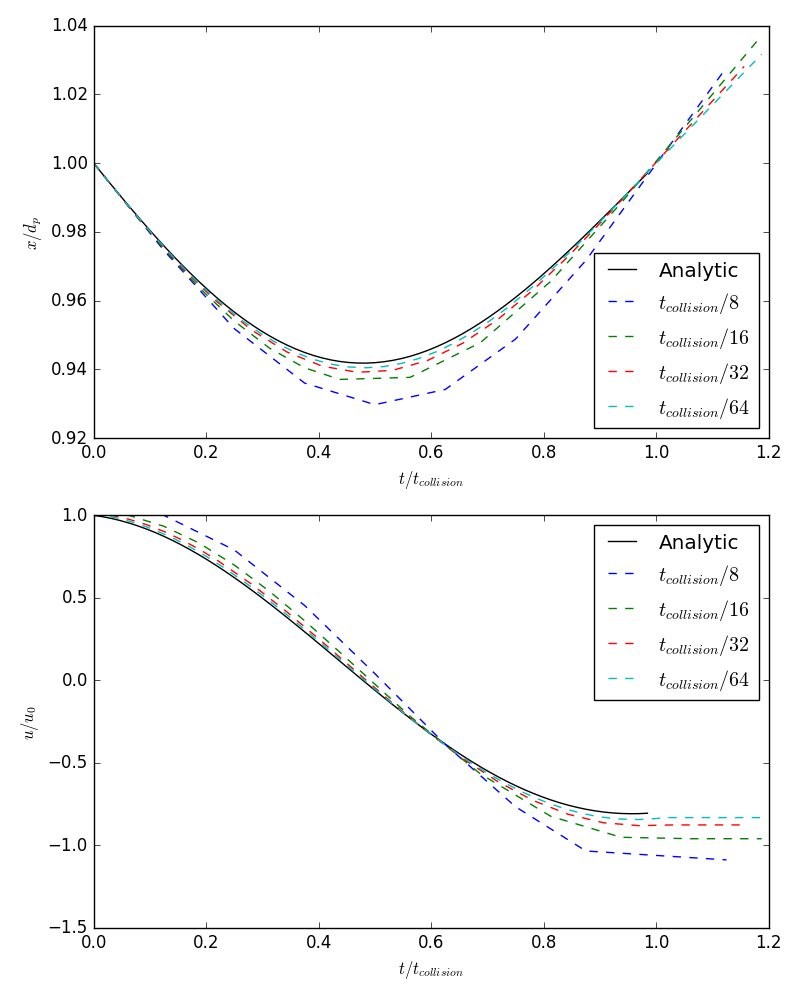
\includegraphics[scale=0.5]{figures/normal_force_verification.png}
\caption{Normalized position and speed against time during a normal collision.}
\label{fig:normal_force_verification}
\end{figure}
\subsection{Friction Force}
The analytic solution used in \ref{fig:friction_verification} is a dynamic Coulomb model friction only. Note that the error increases as the timestep decreases. This is caused by the static friction being lower than the dynamic friction and so not slowing the particle down as much.
If the static friction part of the model is removed then the results are those shown in \ref{fig:friction_verification_dynamic_only}. This very closely matches the analytic solution but is less stable.
\begin{figure}[!htb]
\centering
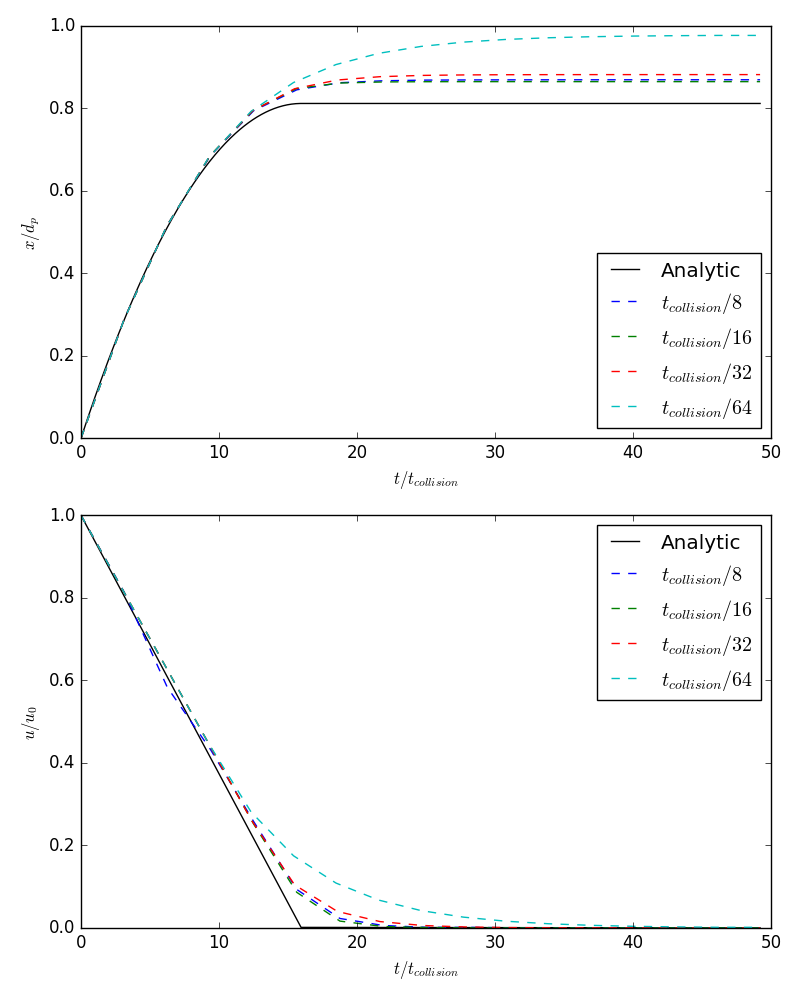
\includegraphics[scale=0.5]{figures/friction_verification.png}
\caption{Normalized position and speed against time during a friction event.}
\label{fig:friction_verification}
\end{figure}
\begin{figure}[!htb]
\centering
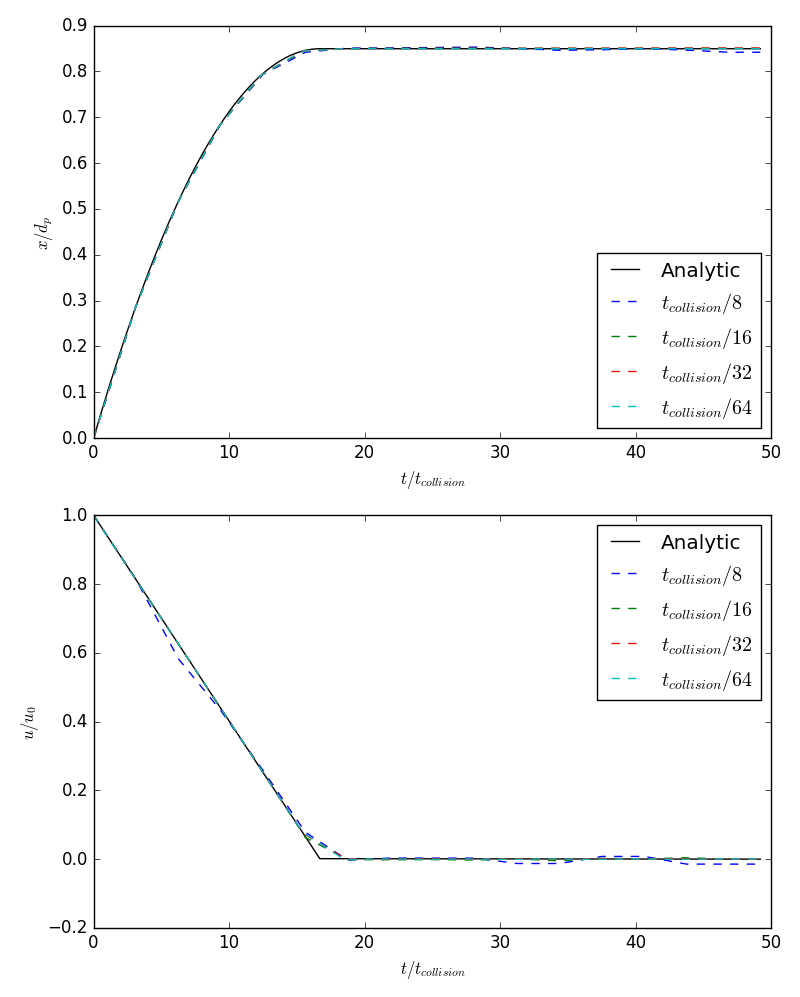
\includegraphics[scale=0.5]{figures/friction_verification_dynamic_only.png}
\caption{Normalized position and speed against time during a friction event with only dynamic friction enabled.}
\label{fig:friction_verification_dynamic_only}
\end{figure}
\subsection{Drag}
\begin{figure}[!htb]
\centering
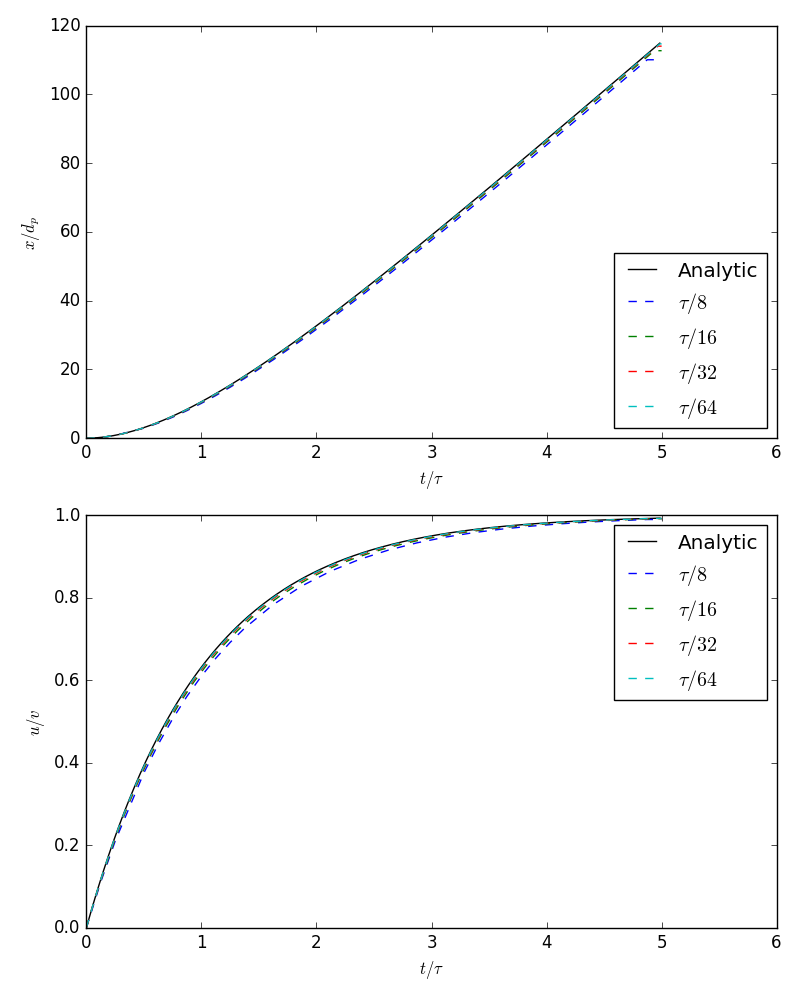
\includegraphics[scale=0.5]{figures/drag_verification.png}
\caption{Normalized position and speed against time of a particle in a moving fluid.}
\label{fig:drag_verification}
\end{figure}
\section{Optimization and Performance}
\textit{This will just contain brief details of optimizations made and analysis of the simulation performance.}
\chapter{Application}
\label{ch:Application}
\textit{General overview of agglomerates and why different properties are interesting.}
\section{Simulation Setup}
\textit{Initial conditions, properties to be varied, how this is defined in the program.}
\subsection{Stoke's Number}
\subsection{Stickyness Number}
The Stickyness Number, Sy, describes how likely particles are to stick to each other through collisions. $L_e$ is the effect length and is usually $d_e - d_b$, where $d_e$ is the effect diameter and $d_b$ is the body diameter. $k_c$ is the cohesion stiffness from equation \ref{eq:cohesion force}. $\epsilon$ is the coefficient of restitution, $u$ is the average particle speed, and $m$ is the average particle mass.

\begin{equation}
Sy = \dfrac{L_e \sqrt{k_c}}{\epsilon \sqrt{L_e^2 k_c + u^2 m}}
\end{equation}

This number is derived from the analytic solution for a normal cohesive collision $<$\textit{TODO: Add section for this in appendix or verification}$>$. When the effect length is $d_e - d_b$ and $u$ is the initial collision speed, the Stickyness Number determines whether the particles will stick after the collision.
\begin{align*}
Sy &< 1 \textit{ Does not stick}
\\ Sy & > 1 \textit{ Sticks}
\end{align*}
\section{Results}
\textit{Presentation of results, graphs etc.}
\section{Discussion}
\textit{Discussion of results including key relationships and conclusions.}
\chapter{Conclusion}
\textit{Overall conclusions from the project. This will likely include some discussion of the successes of the programs as well as a summary of the application results.}
\section{Further Work}
\textit{Recommendations for possible further work from this project.}
\appendix
\chapter{Derivations}
\label{ch:Derivations}
\section{Normal Collision}
\label{der:normal collision}
\begin{align*}
&m \ddot{x} = k_e \delta - \eta \dot{x} \\
&\delta = d_b - x \\
&m \ddot{x} = k_e d_b - k_e x - \eta \dot{x} \\
&m \ddot{x} + \eta \dot{x} + k_e x = d_b k_e \\\\
&\textbf{Complementary Function} \\
&\text{Auxilliary Equation: } mp^2 + \eta p + k_e = 0 \\
&p_{1,2} = \dfrac{- \eta \pm \sqrt{\eta^2 - 4 m k_e}}{2 m} \\
&\text{For this case $\eta ^ 2 > 4 m k_e$ so $p_1$ and $p_2$ are complex.} \\
&\text{Let: } a = \dfrac{-\eta}{2m} \text{ and } b = \dfrac{\sqrt{4mk_e - \eta ^ 2}}{2m} \\
&x = e^{at} (A_1 sin(bt) + A_2 cos(bt)) \\\\
&\textbf{Particular Integral} \\
&\text{Ansatz: } x = B \\
&\dot{x} = \ddot{x} = 0 \\
&k_e B = d_b k_e \\
&B = d_b \\
&x = d_b \\\\
&\textbf{General Solution} \\
&x = e^{at} (A_1 sin(bt) + A_2 cos(bt)) + d_b \\\\
&x(0) = d_b = A_2 + d_b \\
&A_2 = 0 \\\\
&\dot{x}(0) = u_0 = A_1 b \\
&A_1 = \dfrac{u_0}{b} \\\\
&x = e^{at} \dfrac{u_0}{b} sin(bt) + d_b \\
&\dot{x} = u_0 e^{at} (\dfrac{a}{b} sin(bt) + cos(bt))
\end{align*}
\section{Collision Duration}
\label{der:collision duration}
The duration of a collision is considered to be the time for which the particles' body surfaces are touching. For the normal collision used in section \ref{der:normal collision} this is from $t = 0$ until some $t_{col}$ when the moving particle returns to its starting position.
\begin{align*}
&\text{Let: } a = \dfrac{-\eta}{2m} \text{ and } b = \dfrac{\sqrt{4mk_e - \eta ^ 2}}{2m} \\
&x = e^{at} \dfrac{u_0}{b} sin(bt) + d_b \\
&\text{At $t = t_{col}$, $x = d_b$} \\
&e^{a t_{col}} \dfrac{u_0}{b} sin(b t_{col}) = 0 \\
&sin(bt_{col}) = 0 \\
&t_{col} = \dfrac{sin^{-1}(0)}{b} \\
&t_{col} = \dfrac{0 + n \pi}{b} = \dfrac{n \pi}{b} \text{ , } n \in \mathbb{Z} \\
&n = 0 \text{ Initial conditions.} \\
&n = 1 \text{ First crossing after collision, physical result for $t_{col}$.} \\
&t_{col} = \dfrac{\pi}{b} = \dfrac{2 \pi m}{\sqrt{4 m k_e - \eta ^ 2}}\\
\end{align*}
\section{Coefficient of Restitution}
The coefficient of restitution, $\epsilon$, is the ratio of the speeds before ($u_0$) and after ($u_1$) the collision. Since the $x$ velocity after the collision is in the opposite direction to the $x$ velocity before the collision, $\epsilon = \dfrac{- u_1}{u_0}$. The velocity after the collision is determined by finding the velocity at $t = t_{col}$ where $t_{col}$ is the collision duration determined in section \ref{der:collision duration}.
\begin{align*}
&\text{From section \ref{der:normal collision}: } \dot{x} = u_0 e^{at} (\dfrac{a}{b} sin(bt) + cos(bt)) \\
&\text{From section \ref{der:collision duration}: } t_{col} = \dfrac{\pi}{b} \\
&u_1 = u_0 e^{at_{col}} (\dfrac{a}{b} sin(bt_{col}) + cos(bt_{col})) \\
&u_1 = u_0 e^{a \pi / b} (\dfrac{a}{b} sin(\pi) + cos(\pi)) \\
&u_1 = - u_0 e^{a \pi / b} \\
&\epsilon = \dfrac{- u_1}{u_0} = \dfrac{u_0 e^{a \pi / b}}{u_0} = e^{a \pi / b} \\\\
&\text{To determine the damping coefficient for a given $\epsilon$:} \\
&ln(\epsilon) = \dfrac{a \pi}{b} = \dfrac{- \eta \pi}{\sqrt{4 m k_e - \eta^2}} \\
&\eta^2 = \dfrac{4 m k_e ln(\epsilon)^2}{\pi^2 + ln(\epsilon)^2} \\
&\eta = \pm \sqrt{\dfrac{4 m k_e ln(\epsilon)^2}{\pi^2 + ln(\epsilon)^2}} \\
&\text{$\eta$ must be +ve, $ln(\epsilon)$ is -ve so we take the -ve square root.} \\
&\eta = - \sqrt{\dfrac{4 m k_e ln(\epsilon)^2}{\pi^2 + ln(\epsilon)^2}} 
 = - 2 ln(\epsilon) \sqrt{\dfrac{m k_e}{\pi^2 + ln(\epsilon)^2}} \\
&\text{This equation matches the one found in Tuley\cite{tuley}.}
\end{align*}
\section{Normal Collision with Cohesion}
\label{der:normal collision with cohesion}
A normal collision with cohesion has three regimes.
\begin{align*}
&m\dfrac{du}{dt} = 0 \text{ for } x > d_e \\
&m\dfrac{du}{dt} = - k_c \delta_e \text{ for } d_e > x > d_b \\
&m \dfrac{du}{dt} = m \ddot{x} = k_e \delta_b - \eta \dot{x} - k_c \delta_e \text{ for } x < d_b \\
\end{align*}
Two important definitions are those of body overlap ($\delta_b$) and effect overlap ($\delta_e$).
\begin{align*}
&\delta_b = d_b - x \\
&\delta_e = d_e - x \\
\end{align*}
\subsection{Cohesion Only, Incoming ($d_e > x > d_b, u < 0$)}
\begin{align*}
&m \ddot{x} = - k_c \delta_e = - k_c (d_e - x) \\
&m \ddot{x} - k_c x = - k_c d_e \\\\
&\textbf{Complementary Function} \\
&\text{Auxilliary Equation: } mp^2 - k_c = 0 \\
&p = \pm \sqrt{\dfrac{k_c}{m}} \\ 
&x = A_1 e^{t \sqrt{k_c / m}} + A_2 e^{- t \sqrt{k_c / m}} \\\\
&\textbf{Particular Integral} \\
&\text{Ansatz: } x = B \\
&\dot{x} = \ddot{x} = 0 \\
&- k_c x = - k_c d_e  \\
&- k_c B = - k_c d_e \\
& B = d_e \\\\
&\textbf{General Solution} \\
&x = A_1 e^{t \sqrt{k_c / m}} + A_2 e^{- t \sqrt{k_c / m}} + d_e \\
&\dot{x} = \sqrt{\dfrac{k_c}{m}} A_1 e^{t \sqrt{k_c / m}} - \sqrt{\dfrac{k_c}{m}} A_2 e^{- t \sqrt{k_c / m}} \\\\
&x(0) = d_e = A_1 + A_2 + d_e \\
&A_1 = - A_2 \\\\
&\dot{x}(0) = u_0 = \sqrt{\dfrac{k_c}{m}} A_1 - \sqrt{\dfrac{k_c}{m}} A_2 \\
&A_1 = \dfrac{u_0}{2} \sqrt{\dfrac{m}{k_c}} \\\\
&x = \dfrac{u_0}{2} \sqrt{\dfrac{m}{k_c}} e^{t \sqrt{k_c / m}} - \dfrac{u_0}{2} \sqrt{\dfrac{m}{k_c}} e^{- t \sqrt{k_c / m}} + d_e \\
&\dot{x} = \dfrac{u_0}{2} e^{t \sqrt{k_c / m}} + \dfrac{u_0}{2} e^{- t \sqrt{k_c / m}} 
\end{align*}
Two important results from this solution are the impact time ($t_i$) and impact velocity ($u_i$).
\subsubsection{Impact Time ($t_i$)}
\begin{align*}
&\text{At impact: } x = d_b \\
&d_b = \dfrac{u_0}{2} \sqrt{\dfrac{m}{k_c}} e^{t_i \sqrt{k_c / m}} - \dfrac{u_0}{2} \sqrt{\dfrac{m}{k_c}} e^{- t_i \sqrt{k_c / m}} + d_e \\
&\dfrac{2(d_b - d_e)}{u_0} \sqrt{\dfrac{k_c}{m}} = e^{t \sqrt{k_c / m}} - e^{-t \sqrt{k_c / m}}  = 2 sinh(\sqrt{\dfrac{k_c}{m}} t) \\
&t_i = \sqrt{\dfrac{m}{k_c}} sinh^{-1}\Bigg(\dfrac{d_b - d_e}{u_0} \sqrt{\dfrac{k_c}{m}}\Bigg)
\end{align*}
\subsubsection{Impact Velocity ($u_i$)}
\begin{align*}
&u_i = \dfrac{u_0}{2} e^{t_i \sqrt{k_c / m}} + \dfrac{u_0}{2} e^{- t_i \sqrt{k_c / m}} \\
\end{align*}
\subsection{Full Contact ($x < d_b$)}
\begin{align*}
&m \dfrac{du}{dt} = m \ddot{x} = k_e \delta_b - \eta \dot{x} - k_c \delta_e \\
&m\ddot{x} + \eta \dot{x} + (k_e - k_c) x = k_e d_b - k_c d_e \\\\
&\textbf{Complementary Function} \\
&\text{Auxilliary Equation: } mp^2 + \eta p + k_e - k_c = 0 \\
&p_{1,2} = \dfrac{- \eta \pm \sqrt{\eta^2 - 4m(k_e - k_c)}}{2 m} \\
&\text{For this case $k_e > k_c$ and $\eta ^ 2 > 4 m (k_e - k_c)$ so $p_1$ and $p_2$ are complex.} \\
&\text{Let: } a = \dfrac{-\eta}{2m} \text{ and } b = \dfrac{\sqrt{4mk_e - \eta ^ 2}}{2m} \\
&x = e^{at} (A_1 sin(bt) + A_2 cos (bt)) \\\\
&\textbf{Particular Integral} \\
&\text{Ansatz: } x = B \\
&\dot{x} = \ddot{x} = 0 \\
&(k_e - k_c)B = k_e d_b - k_c d_e \\
& B = \dfrac{k_e d_b - k_c d_e}{k_e - k_c} \\\\
&\textbf{General Solution} \\
&x = e^{at} (A_1 sin(bt) + A_2 cos (bt)) + \dfrac{k_e d_b - k_c d_e}{k_e - k_c} \\
&\dot{x} = e^{at}((A_1 a - A_2 b)sin(bt) + (A_1 b + A_2 a) cos(bt)) \\\\
&\text{To simplify the result the $t$ here is $t - t_i$ in the overall collision.} \\
&x(0) = d_b \\
&A_2 + \dfrac{k_e d_b - k_c d_e}{k_e - k_c} = d_b \\
&A_2 = \dfrac{k_c (d_e - d_b)}{k_e - k_c} \\\\
&\text{Let: } c = \dfrac{k_c (d_e - d_b)}{k_e - k_c} \\\\
&\dot{x}(0) = aA_2 + bA_1 = u_i \\
&A_1 = \dfrac{u_i - aA_2}{b} = \dfrac{u_i - ac}{b} \\\\
&x = e^{at} (\dfrac{u_i - ac}{b} sin(bt) + c cos (bt)) + \dfrac{k_e d_b - k_c d_e}{k_e - k_c} \\
&\dot{x} = e^{at}\Big(\Big(\dfrac{u_i - ac}{b} a - \dfrac{k_c (d_e - d_b)}{k_e - k_c} b\Big)sin(bt) + \Big(\dfrac{u_i - ac}{b} b + \dfrac{k_c (d_e - d_b)}{k_e - k_c} a\Big) cos(bt)\Big) \\\\
\end{align*}
The position cannot be analytically solved for $t$ in order to find the initial return velocity. A reasonable estimation for this is to use $t_{col} = \dfrac{\pi}{b}$, and other results, from section \ref{der:normal collision}. Thus the initial return velocity, $u_r$, can be found to be $u_r = - \epsilon u_i$.
\subsection{Cohesion Only, Returning ($d_e > x > d_b, u > 0$)}
The General Solution to the returning equation is the same as the incoming equation.
\begin{align*}
&\textbf{General Solution} \\
&x = A_1 e^{t \sqrt{k_c / m}} + A_2 e^{- t \sqrt{k_c / m}} + d_e \\
&\dot{x} = \sqrt{\dfrac{k_c}{m}} A_1 e^{t \sqrt{k_c / m}} - \sqrt{\dfrac{k_c}{m}} A_2 e^{- t \sqrt{k_c / m}} \\\\
&\text{To simplify the result the $t$ here is $t - t_r$ in the overall collision where $t_r$ is the return time.} \\
&x(0) = d_b = A_1 + A_2 + d_e \\
&A_1 + A_2 = (d_b - d_e)\\\\
&\dot{x}(0) = u_r = \sqrt{\dfrac{k_c}{m}} A_1 - \sqrt{\dfrac{k_c}{m}} A_2 \\
&A_1 = \dfrac{1}{2}\Big(d_b - d_e + u_r \sqrt{\dfrac{m}{k_c}} \Big) \\
&A_2 = \dfrac{1}{2}\Big(d_b - d_e - u_r \sqrt{\dfrac{m}{k_c}} \Big) \\
&A_1 = \dfrac{u_0}{2} \sqrt{\dfrac{m}{k_c}} \\\\
&x = \dfrac{1}{2}(d_b - d_e)(e^{t \sqrt{k_c / m}} + e^{- t \sqrt{k_c / m}}) + \dfrac{1}{2}u_r\sqrt{\dfrac{m}{k_c}}(e^{t \sqrt{k_c / m}} - e^{-t \sqrt{k_c / m}}) + d_e \\
&x = (d_b - d_e)cosh\Big(\sqrt{\dfrac{k_c}{m}} t\Big) + u_r \sqrt{\dfrac{m}{k_c}} sinh\Big(\sqrt{\dfrac{k_c}{m}}t\Big) + d_e \\
&\dot{x} = \sqrt{\dfrac{k_c}{m}}(d_b - d_e)sinh\Big(\sqrt{\dfrac{k_c}{m}} t\Big) + u_r cosh\Big(\sqrt{\dfrac{k_c}{m}}t\Big) + d_e \\
\end{align*}
\section{Stickyness Number}
Taking the results from section \ref{der:normal collision with cohesion} it is known that if the particle is to escape the collision the position, $x$, will at some point return to $d_e$. Thus:
\begin{align*}
&d_e = (d_b - d_e)cosh\Big(\sqrt{\dfrac{k_c}{m}} t\Big) + u_r \sqrt{\dfrac{m}{k_c}} sinh\Big(\sqrt{\dfrac{k_c}{m}}t\Big) + d_e \\
&(d_b - d_e)cosh\Big(\sqrt{\dfrac{k_c}{m}} t\Big) + u_r \sqrt{\dfrac{m}{k_c}} sinh\Big(\sqrt{\dfrac{k_c}{m}}t\Big) = 0 \\
&tanh(\sqrt{\dfrac{k_c}{m}} t) = \dfrac{d_e - d_b}{u_r \sqrt{\dfrac{m}{k_c}}} \\
&\text{This only has a solution when the RHS is less than 1.} \\
&\text{Thus, for a particle to stick in a collision:} \\
&\dfrac{d_e - d_b}{u_r}\sqrt{\dfrac{k_c}{m}} > 1 \\
&u_r = -\epsilon u_i \\
&u_i = u_0 cosh\Big(t_i \dfrac{k_c}{m}\Big) = u_0 cosh\Big(sinh^{-1}\Big(\dfrac{d_b - d_e}{u_0}\sqrt{\dfrac{k_c}{m}}\Big)\Big) \\
&\dfrac{d_e - d_b}{u_r}\sqrt{\dfrac{k_c}{m}} = \dfrac{d_e - d_b}{-\epsilon u_0 cosh\Big(sinh^{-1}\Big(\dfrac{d_b - d_e}{u_0}\sqrt{\dfrac{k_c}{m}}\Big)\Big)}\sqrt{\dfrac{k_c}{m}} \\
&\dfrac{d_e - d_b}{u_r}\sqrt{\dfrac{k_c}{m}} = \dfrac{(d_b - d_e)\sqrt{k_c}}{\epsilon \sqrt{(d_b - d_e)^2 k_c + u_0 ^ 2 m}} \\\\
&\text{Finding the dimensions of this number:} \\
&\text{Dimensions of stiffness: } [M][L][T]^{-2}[L]^{-1} = [M][T]^{-2} \\
&\dfrac{[L]([M][T]^{-2})^{0.5}}{[1]([L]^2[M][T]^{-2} + [L]^2[T]^{-2}[M])^{0.5}} \\
& = \dfrac{[L][M]^{0.5}[T]^{-1}}{[L][T]^{-1}[M]^{0.5}} = [1] \\
&\text{This shows that the number is dimensionless.}
\end{align*}
\section{Dynamic Friction Sliding}
\begin{align*}
&F_n = mg \\
&F_t^{dynamic} = - \mu |F_n| \\
&\dfrac{du}{dt} = \ddot{x} = \dfrac{- \mu m g}{m} = - \mu g\\
&\dot{x} = - \mu g t + u_0 \\
&x = \dfrac{- \mu g}{2}t^2 + u_0 t + x_0 \\
\end{align*}
\section{Particle Drag}
\begin{align*}
&m\dfrac{du}{dt} = \dfrac{m}{\tau}(u_f - u) \\
&\ddot{x} + \dfrac{1}{\tau} \dot{x} = \dfrac{u_f}{\tau} \\\\
&\textbf{Complementary Function} \\
&\text{Auxilliary Equation: } p^2 + \dfrac{1}{\tau}p = 0 \\
&p_1 = 0, p_2 = - \dfrac{1}{\tau} \\
&x = A_1e^{0t} + A_2e^{-t/\tau} \\\\
&\textbf{Particular Integral} \\
&\text{Ansatz: } x = Bt \\
&\dot{x} = B \\
&\ddot{x} = 0 \\
&\dfrac{B}{\tau} = \dfrac{u_f}{\tau} \\
&B = u_f \\\\
&\textbf{General Solution} \\
&x = A_1 + A_2 e^{-t /\tau} + u_f t \\
&\dot{x} = \dfrac{-A_2}{\tau} e^{-t/\tau} + u_f \\\\
&x(0) = 0 = A_1 + A_2 \\
&\dot{x}(0) = 0 = \dfrac{-A_2}{\tau} + u_f \\
&A_2 = u_f \tau \\
&A_1 = - u_f \tau \\\\
&x = u_f \tau (e^{-t/\tau} - 1) + u_f t \\
&\dot{x} = u_f (1 - e^{-t/\tau}) \\
\end{align*}
\bibliography{references}
\bibliographystyle{unsrt}
\end{document}
